\section{Interview mit einem Fachmann}
\subsection{Idee}
Es sollte ein Interviewvideo mit einem passionierten Medientechniklehrer gedreht werden, um den Usern, der erstellten Plattform, einen tiefen Einblick in die Medientechnik zu bieten. Dabei wird auch an Fragestellungen aus dem Animationsvideo angeknüpft, jedoch wird auf diese ausführlicher und detailreicher eingegangen. Die Aufnahme bietet durch Verwendung eines Green Screens, eine Reihe an Möglichkeiten das Video spannender und ansprechender zu machen. Der Green Screen wurde genutzt um den Betrachter des Videos begleitend zu den Aussagen, des Fachmanns mit visuellen Beispielen zu unterstützen.
\subsection{Dreh}
\renewcommand{\kapitelautor}{Autor: Niklas Kienreich}
Bei den Dreharbeiten wurde genau wie bei den anderen Interviewvideos eine Auflösung von 1920 mal 1080 px verwendet und eine Framerate von 25fps. Nähere Infos zu den allgemeinen Aspekten der Videoaufnahmen sind im Kapitel „Technik“ zu finden.
\subsubsection{Aufbau}
\paragraph{Hintergrund}
\leavevmode \\
Was sich jedoch von den anderen Videos stark unterscheidet, war der Aufbau, des Sets. Der Dreh fand in einem Raum statt, in dem keines, der anderen Videos gedreht wurde. Dem Video-Labor, der HTL Rennweg. Dieser Raum stellte einiges an Equipment zur Verfügung. Unter anderem eine grüne Papierrolle, die man herabziehen und als Green Screen verwenden konnte. Diese deckte aber nicht den gesamten Hintergrund ab, also wurde auf den Grünen Vorhang ausgewichen, der sich an einer Wand, des Raumes befand. Das Problem hier war es, den Vorhang faltenlos zu spannen, da die Umsetzung eines Green Screens keine starke Schattenbildung toleriert. Das heißt, dass der Vorhang umständlich mit Klemmen befestigt wurde damit die Fläche, die sich auf der Aufnahme befand, so flach wie möglich war.

\begin{figure}[H] 
  \centering
     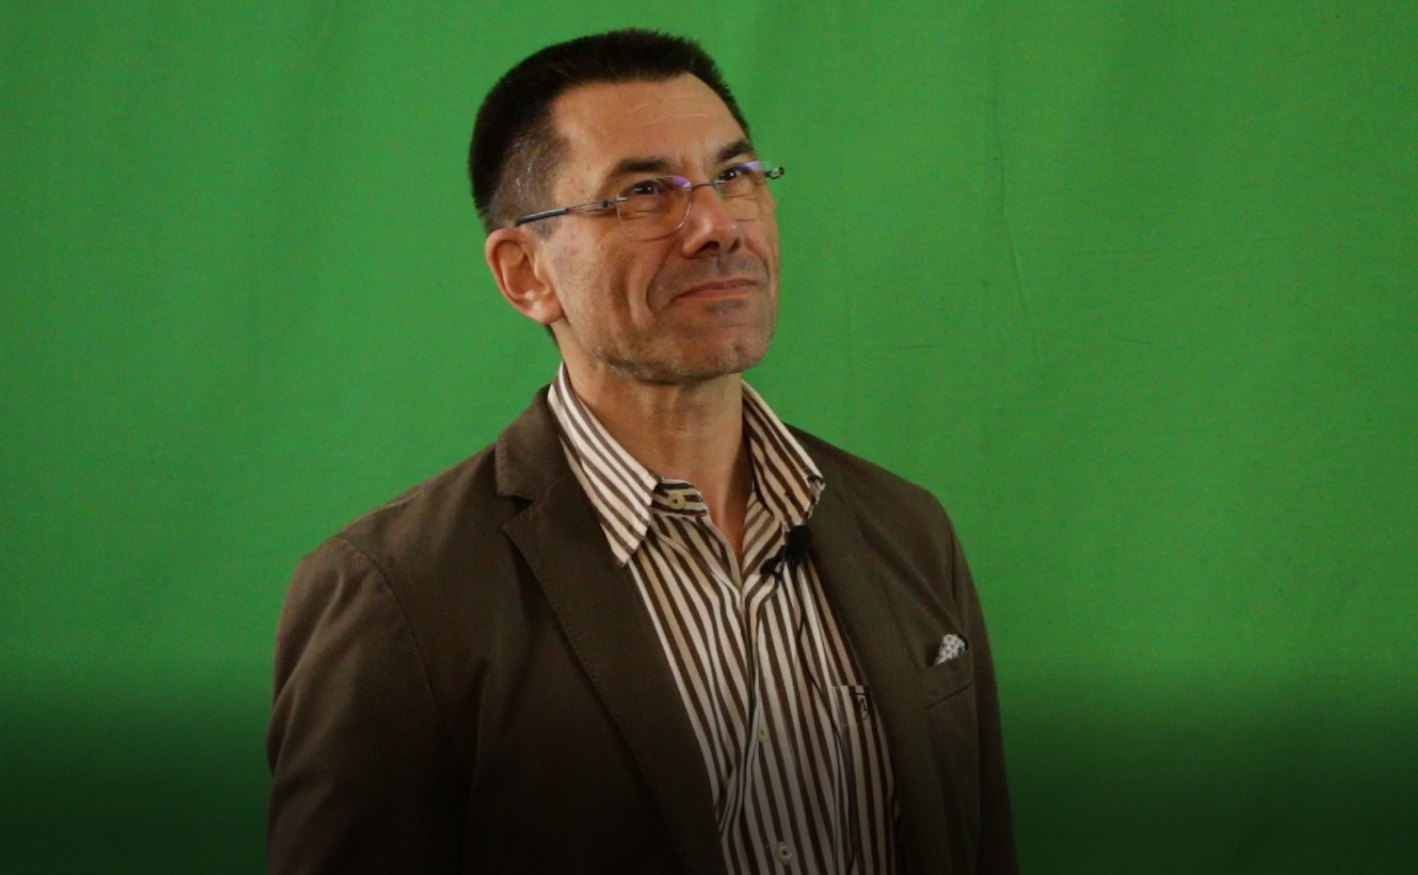
\includegraphics[width=0.7\textwidth]{video_abb1.png}
  \caption{Aufnahme des Fachmanns vor Green Screen}
\end{figure}

\paragraph{Beleuchtung}
\leavevmode \\
Auch die Beleuchtung war anders, als bei den anderen Aufnahmen. Zu Beginn gab es drei Punkte auf die geachtet wurde:
\begin{itemize}
\item Keine Schatten auf dem Green Screen
\item Keine Reflexionen in der Brille, des Fachmanns
\item Der Fachmann selbst ist gut beleuchtet 
\end{itemize}
Bei dem Aufbau wurde der Interviewte möglichst weit weg vom Green Screen aufgestellt und eine Softbox wurde bei dem Führungslicht verwendet. Diese beiden Faktoren sorgten dafür, dass auf die grüne Fläche nur ein schwacher, diffuser Schatten geworfen wurde. Zwei Fülllichter, wobei sich eins auf jeder Seite befand, leuchteten den Schatten aus, und glichen gleichzeitig den geworfenen Schatten, des jeweils anderen Fülllichts aus. Das rechte Fülllicht wurde so ausgerichtet, dass es zu keiner Reflexion in einer Brille kam. Der Fachmann wurde so aber leider von dem Licht geblendet, also musste in Kauf genommen werden, dass die Brille leicht reflektiert.
\subsection{Schnitt}
Geschnitten wurde das Video, wie die anderen in Adobe Premiere Pro. Auch beim Schnitt wurde sich an das Schema anderer Videos gehalten, um eine Art Zusammenhang zu vermitteln. Das heißt, dass Fragen als Text-Slides eingeblendet werden, die dann durch Ausschnitte, aus dem Interview beantwortet werden.
\subsubsection{Grobschnitt}
Der Grobschnitt hat sich als kniffelig erwiesen. Das Endprodukt sollte eine maximale Länge von ungefähr Zehn Minuten haben. Bei den Dreharbeiten haben sich aber über eine halbe Stunde Material ergeben. Um das Video kürzer zu machen gab es drei Möglichkeiten. Das Wegschneiden, der gestellten Fragen, da diese durch die Slides ersetzt wurden, war die Erste. Die Zweite war es, Fragen die nicht als zu wichtig erachtet wurden, nicht in das Video aufzunehmen. Die letzte und schwierigste Möglichkeit, war es die Antworten, des Fachmanns zu kürzen. Der Grund, aus dem dies so schwer war, war dass der Fachmann sehr lange Antworten gab und viele seiner Sätze einen Aufbau, für folgende Sätze bildeten. Dementsprechend hat diese Option relativ wenig Verwendung im Schnitt gefunden.
\subsubsection{Feinschnitt}
Beim Feinschnitt, wurden die Übergänge auf die Frage-Slides eingearbeitet. Hier wurde ganz einfach mit Layern und Opazität gearbeitet. Die Videospur mit dem Fachmann lief auf dem vordersten Layer. Wenn sich eine Antwort dem Ende näherte wurde ab einem gewissen Frame, einem sogenannten Keyframe, bis zu einem weiteren Keyframe, die Opazität gleichmäßig von 100 Prozent auf null herabgesenkt. Mit derselben Methode wurden die Slides daraufhin ein- und wieder ausgeblendet. Keyframes sind aber nicht nur für visuelle Effekte verwendbar. Auch die Lautstärke, der Hintergrundmusik wurde so immer wieder erhöht und wieder herabgesenkt.\cite{keyframes}
\subsection{Green Screen}
Um den Green Screen in Premiere Pro zu verwenden, muss man unter den Keying-Effekten den sogenannten Ultra Key auswählen. Dieser erlaubt es einen gewissen Teil, des Farbspektrums durchsichtig zu machen, damit ein Bild oder Video auf der hinteren Ebene sichtbar wird. Dieser Effekt ist gut für Hintergründe und sehr beliebt bei den Wettervorhersagen. Das helle Grün wird deshalb meist verwendet, da es eine Farbe ist, die in der Natur selten vorkommt, und somit sehr unwahrscheinlich, unabsichtlich am Drehort auftaucht. Sobald der Ultra Key auf das Videomaterial angewandt wird, wählt man mit einer Pipette die Farbe Grün aus. Da es bei dem Video mit dem Fachmann leichte Schatten auf dem Grün gab, musste die Effektoption „aggressiv“ gewählt werden, damit das grüne Farbspektrum mehr Toleranz hergibt. Dann wurde ein Grünton zwischen Schatten und Licht gewählt, der jeden anderen im Video erfasste. Dies war ein bisschen kniffelig, hat aber nicht allzu lange gedauert. Mit weiteren Einstellungen, des Ultra Keys, wurden die Kanten des Fachmanns abgeschwächt, so dass das Video ein natürlicheres Aussehen hatte.\cite{ultra}

\begin{figure}[H] 
  \centering
     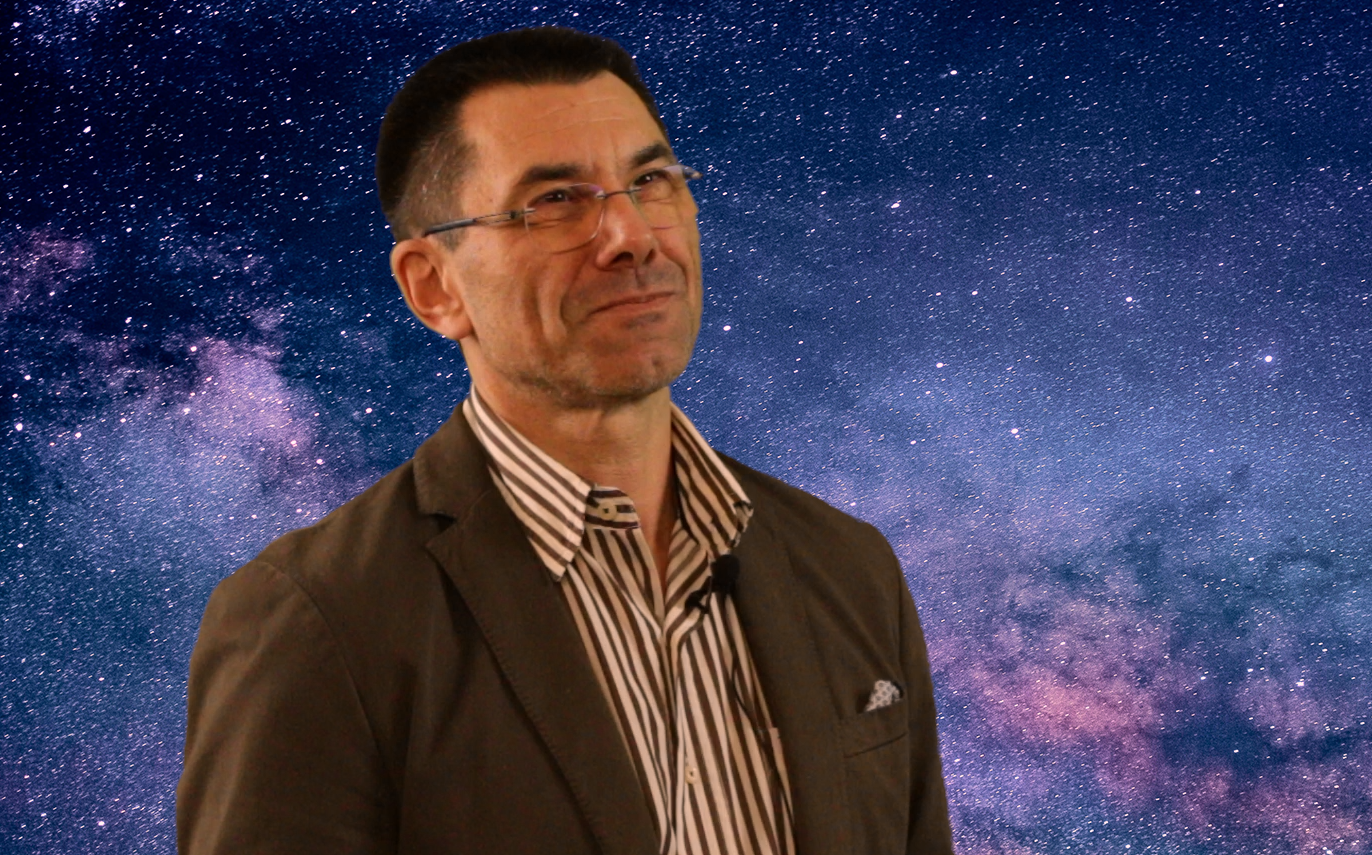
\includegraphics[width=0.7\textwidth]{video_abb2.png}
  \caption{Aufnahme mit verändertem Hintergrund}
\end{figure}

\subsection{Herausforderungen}
Bei der Aufnahme, dürfte ein zu hoher ISO-Wert verwendet worden sein, denn bei dem Video ergab sich ein relativ starkes Bildrauschen.\cite{iso} Dieses Problem hat sich jedoch selbst gelöst, nachdem der Großteil, der Bildfläche mit dem Ultra-Key enfernt wurde. Das Rauschen auf dem Fachmann selbst, fiel kaum auf und konnte somit unbehandelt bleiben. Aber auch das Audio war nicht optimal. Die Lautstärke schwankte stark. Also wurde ein sogenannter Kompressor verwendet, um leisere Töne lauter und lautere Töne leiser zu machen.\cite{kompressor}


\chapter{Animationsvideo}
\section{Idee}
\renewcommand{\kapitelautor}{Autor: Niklas Kienreich}
Das Animationsvideo sollte als Eyecatcher für die Zielgruppe dienen. Der Gedanke war, Allgemeines über die HTL auf möglichst witzige, ansprechende Weise zu vermitteln. Die Animation schafft das besser, als die restlichen Videos, da man sich bei den Interviews auf eine lockere, aber doch ernste, zielführende Gesprächsführung verlassen hat. Eine Frage die man sich nun aber stellen musste war, wie man das Video animiert. Neben vier Videos, die nicht nur gedreht, sondern auch geschnitten und farbkorrigiert werden mussten und der Website, war für so ein kleines Team von drei Personen nicht allzu viel Zeit eingeplant. Nach überraschend kurzer Recherche, war nicht nur eine einfache, sondern auch ansprechende Lösung gefunden. In den letzten Jahren haben immer mehr Kanäle auf Youtube bei unserer Zielgruppe großes Interesse geweckt. Laut Youtube existiert einer der beliebteren Kanäle seit dem 30.08.2014 und hat seitdem knapp über 6 Millionen Abonnenten und 900 Millionen Aufrufe gesammelt.\cite{channel} Ihre Videos sind kurze Animationen im vereinfachten Stil. Also keine flüssigen Bewegungen, sondern mehr sprunghafte Frames mit einem Voice-Over. Es erinnert an eine digitale Version eines so genannten „Draw my life“.
\section{Ziel}
\renewcommand{\kapitelautor}{Autor: Niklas Kienreich}
Das Ziel war es, mit dem zwar kürzesten, aber unterhaltsamsten Video, die wichtigsten, grundlegenden Informationen zu Höheren Technische Bundeslehranstalten zu bieten. Die detaillierten Informationen zu der Schule selbst, sind im Interviewvideo mit dem Abteilungsvorstand zu finden. Die User sollten nach den beiden Videos zuerst wissen, ob sie an solch einer Schule überhaupt Interesse haben. Ein Wissen das essenziell ist, bevor man sich auf die Frage stürzt, ob die Medientechnik, oder gar irgendein anderer technischer Fachbereich für einen geeignet ist.
\section{Drehbuch}
\renewcommand{\kapitelautor}{Autor: Niklas Kienreich}
\subsection{Brainstorming}
Bevor das Drehbuch geschrieben werden konnte, musste ein Brainstorming durchgeführt werden. Hierbei wurden zuerst die Drehbücher beziehungsweise Fragen, der anderen Videos herangezogen, um zu ermitteln, welche Fragen noch nicht geklärt wurden, oder welche Fragestellung man nochmal genau herausheben sollte.
\leavevmode \\
Das Brainstorming brachte folgende Ergebnisse:
\begin{itemize}
\item Was genau ist eine HTL?
\item Welche Fachbereiche gibt es und wie teilen sie sich auf?
\item Was lernt man an der Schule unter anderem?
\item Was für Möglichkeiten bieten sich einem nach der Schule?
\end{itemize}
Anhand dieser Punkte, wurde ein Drehbuch geschrieben, zu dem dann noch zusätzlich ein Storyboard entworfen wurde, damit die Umsetzung möglichst reibungslos verlaufen sollte.
\subsection{Eindruck}
Da das Animationsvideo als einleitendes Video genutzt wird, ist es sehr wichtig, wie es auf den Benutzer wirkt. Um das Video freundlich, einladend und möglichst natürlich wirken zu lassen, wurde beschlossen, dass es in dem Video um einen Schüler geht, mit dem sich der User identifizieren kann.
\section{Audioaufnahme}
\subsection{Dämmung}
Das Audio wurde im Audio-Labor, der Schule aufgenommen. Das Tonstudio, dass sich dort befindet ist mit Schaumstoff ausgepolstert. Dies hat den Zweck, die Akustik innerhalb des Raumes zu verbessern, indem der Schaumstoff Hall dämpft. Das Material selbst und seine Dicke, können die Effektivität beeinflussen. Zum Beispiel werden bei dünnerer Verkleidung eher höhere Frequenzen gedämpft und keine tiefen. Es ist erstrebenswert Hall so zu verhindern, dass er gleichmäßig über das gesamte Spektrum absorbiert wird.\cite{damm} 
\subsection{Aufnahmesoftware}
Aufgenommen wurden die Audios, für das Animationsvideo und die Website, mit dem Programm Cubase. Es ist eine DAW-Software (Digital Audio Workstation). Mit ihr ist es nicht nur möglich Audiospuren aufzunehmen und sie zu exportieren, sondern man kann Audios auch bearbeiten, mixen und es ist sogar möglich mit dem Programm zu komponieren.\cite{cube}
\subsection{Schnittsoftware}
Der Schnitt, der aufgenommenen Spuren erfolgte jedoch auf dem Programm Audacity. Dieses Programm ist eine kostenlose Open Source Software, für die Aufnahme und Bearbeitung von Audios. Die Bedienung ist schnell und einfach.\cite{auda}
\section{Umsetzung}
\subsection{Zeichnen}
Im Adobe Illustrator wurde ein Dokument mit der Größe 1920 mal 1080 Pixel erstellt. Dies hatte den Zweck, die später exportierten Bilder in ein Full-HD-Video einfügen zu können, ohne dass sie unnötig skaliert werden müssten. In diesem Dokument wurde der Charakter gezeichnet. Bei seinem Design treten vertraute Ähnlichkeiten zum Logo auf. Die offene Stelle an der linken Seite wurde beibehalten und auch beim Charakter übernommen. Bei diesem Entwurf unterschied sich nicht viel zu den bisherigen, im Illustrator erstellten Bildern. Einen wichtigen Unterschied gab es aber doch. Die Augen, der Mund, der Körper und sogar die Schatten befanden sich alle auf anderen Layern. Das hatte den Zweck, dass man einfach nur einen Layer ausblenden und einen anderen einblenden musste, und schon hatte man eine andere Position oder Emotion des Charakters. Also wurden vorab nach Drehbuch und Storyboard, alle verschiedenen Grafiken angefertigt. Darunter auch Schriftzüge und ähnliche Elemente, die man einblenden konnte.

\begin{figure}[H] 
  \centering
     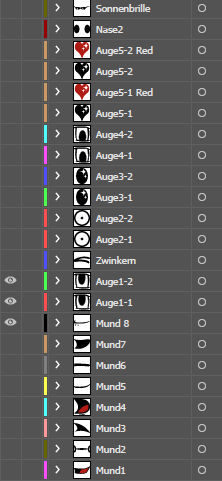
\includegraphics[width=0.25\textwidth]{video_abb3.png}
  \caption{Ein Ausschnitt der Layer-Liste}
\end{figure}

\subsection{Export}
Als alles fertiggezeichnet war, wurde noch einmal das Drehbuch und das Storyboard zur Hand genommen. Nun wurde festgelegt welche Augen, welcher Mund und welche anderen Elemente pro Bild, Satz für Satz benötigt wurde. Dann wurden die benötigten Ebenen für jedes Bild sichtbargemacht und das Bild daraufhin mit zuordnungsbarer Nomenklatur als PNG abgespeichert. PNG wurde gewählt, weil zu dem Zeitpunkt nicht klar war, ob der Charakter auch in andere Videos eingebunden wird und so war PNG, welches Transparenz unterstützt eine gute Wahl als Format.

\begin{figure}[H] 
  \centering
     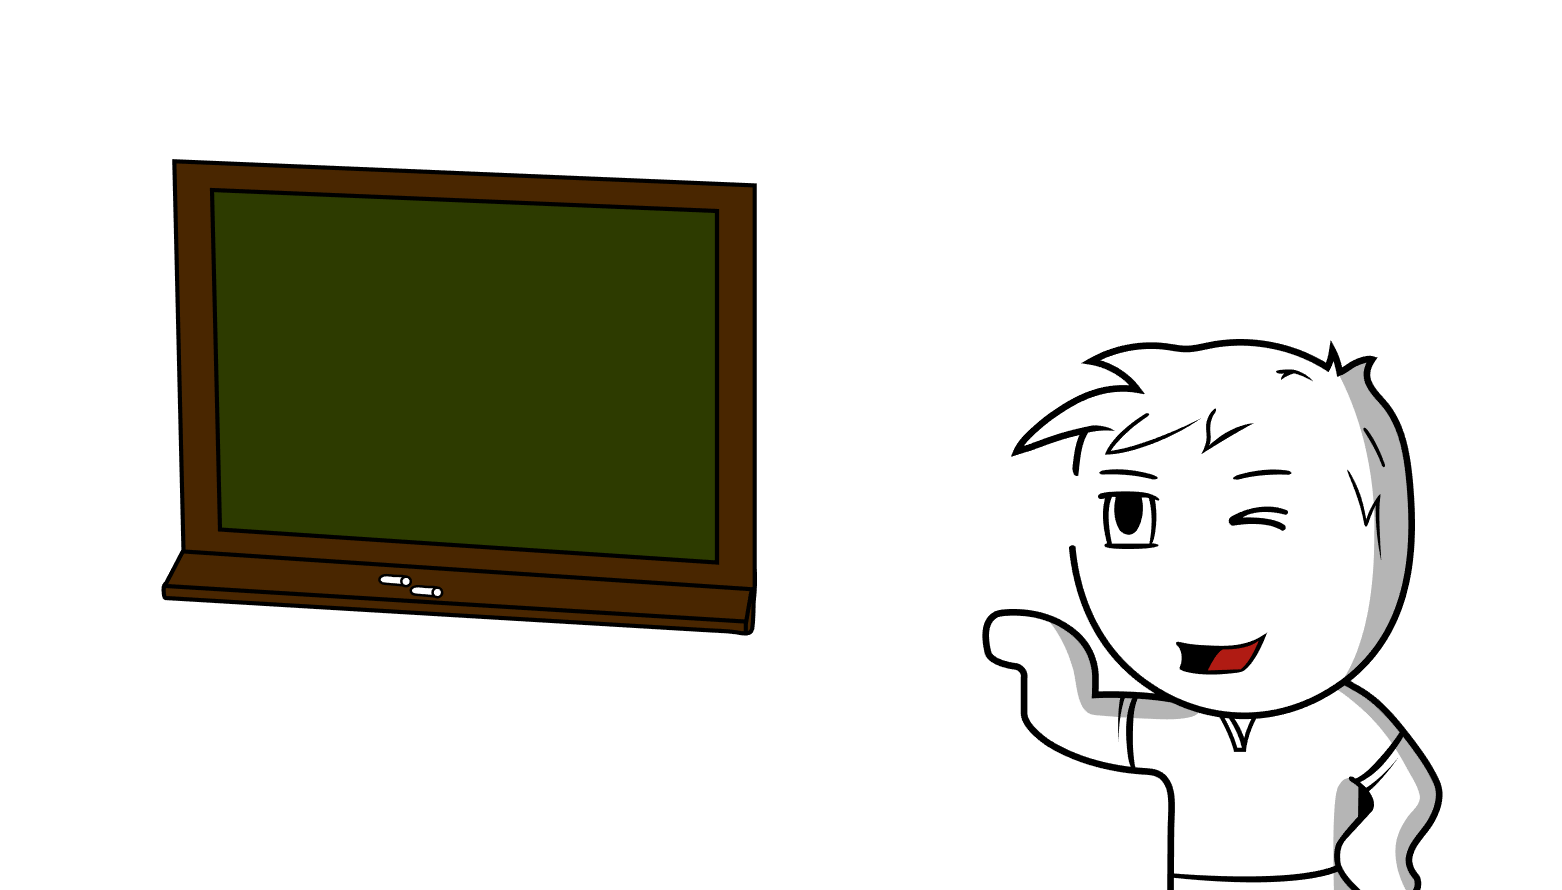
\includegraphics[width=0.7\textwidth]{video_abb4.png}
  \caption{Ein mögliches Bild, zusammengestellt aus mehreren Layern}
\end{figure}

\subsection{Animation}
Die Animation in dem Stop-Motion-Style war grundsätzlich einfach zu animieren. Die Audiospur wurde in Adobe Premiere gezogen, genauso wie die Bilder in der bereits festgelegten Reihenfolge. Ihre Framezahl, beziehungsweise wie lange die Bilder zu sehen waren, musste nur noch an das Audio angepasst werden.

